%about objects not information; we can discuss in outside the box the issue of
%information needed forver but shuttled in and out.

\chapter{Extreme Scalability of Long-lived Data}
\label{chapter:large-long-lived}

Sometimes, despite your best efforst of tuning entities and collections, your
application's objects still do not fit into the memory constraints of the target
platform. All of the tuning advice presented so far in this book can only get you
so far. Therefore, even though objects that live forever are free from the bugs
that riddle objects with correlated lifetime, managing a great number of
long-lived objects nevertheless comes with its own challenges. When your objects
don't fit in a given size of Java heap, there are three solutions at your
disposal. 

\paragraph{Throw Hardware At It} The first solution you may consider is buying
more memory for the target platform.

\paragraph{Swap Objects in and Out of the Java Heap}

\paragraph{Break the Java Mold} Despite being an object-oriented language, there
is nothing in the Java language that prevents you from storing objects in a
non-object oriented way --- nothing, that is, except programming time and
maintenance expense. It is possible to store data only in arrays, as one would in
a language such as Fortran, and retain a great deal of object orientation in your
data models and programming interfaces. \autoref{sec:fortran-style} discusses how
to store objects in this ``Fortran style''.

\section{Scalability: Quantitative Methodology}

\begin{figure}
\centering
	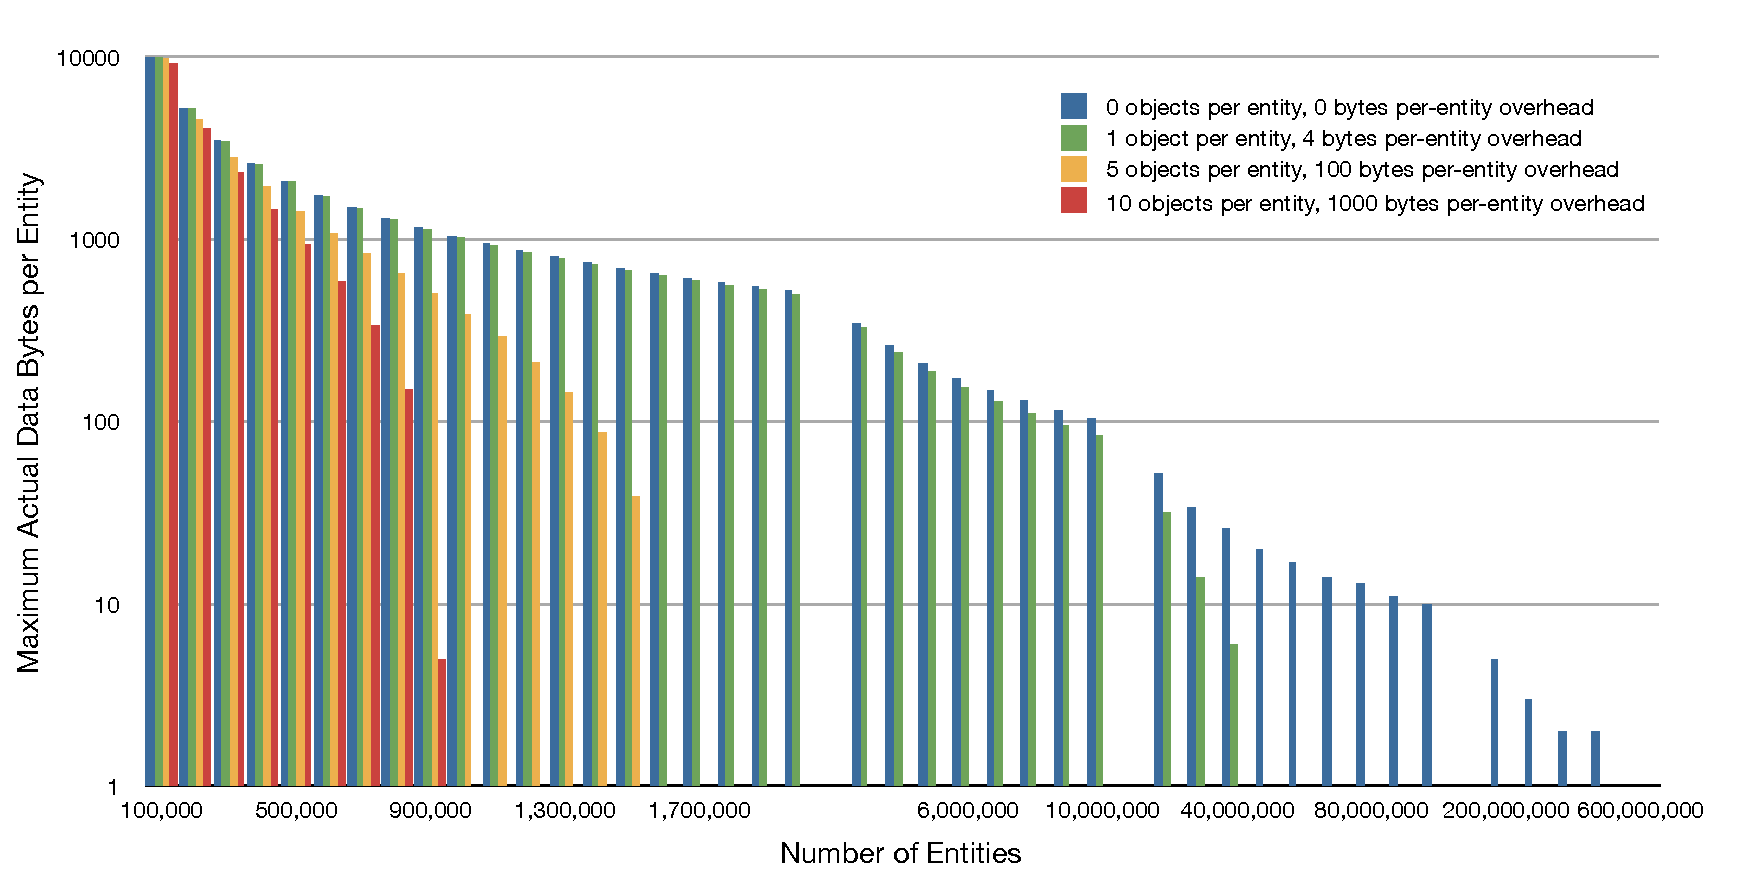
\includegraphics[width=\textwidth]{part4/Figures/maxActualData}
	\caption{The amount of actual data you can store in your entities depends on
	the degree of delegation in your entities, and the per-entry overhead of the collection in which these entities
	reside. This chart assumes a limit of 1 gigabyte of Java heap.}
\end{figure}

\section{An Example: Representing Relationships}

A good starting example for this discussion is a graph of nodes and edges. This
basic data structure is common to many scenarios. For example, when caching
data from a relational database in the Java heap, the entities (rows in a
database table) and relations (columns that contain indices into tables) become
the nodes and edges in a graph.

\begin{example}{Storing a Graph}
Consider a graph composed of nodes and edges, such as the small
example illustrated in  \autoref{fig:exampleGraph}. There are several ways to
implement the abstract data types, of nodes and edges, shown in that figure.
Each strategy has its positives and negatives, depending on whether ease of
maintenance or memory consumption are of primary importance.
If the graph has a great many nodes and edges, you must design the storage
for this graph carefully.
\end{example}

\begin{figure}
\centering
\subfigure[Example graph.]{
\shortstack{
	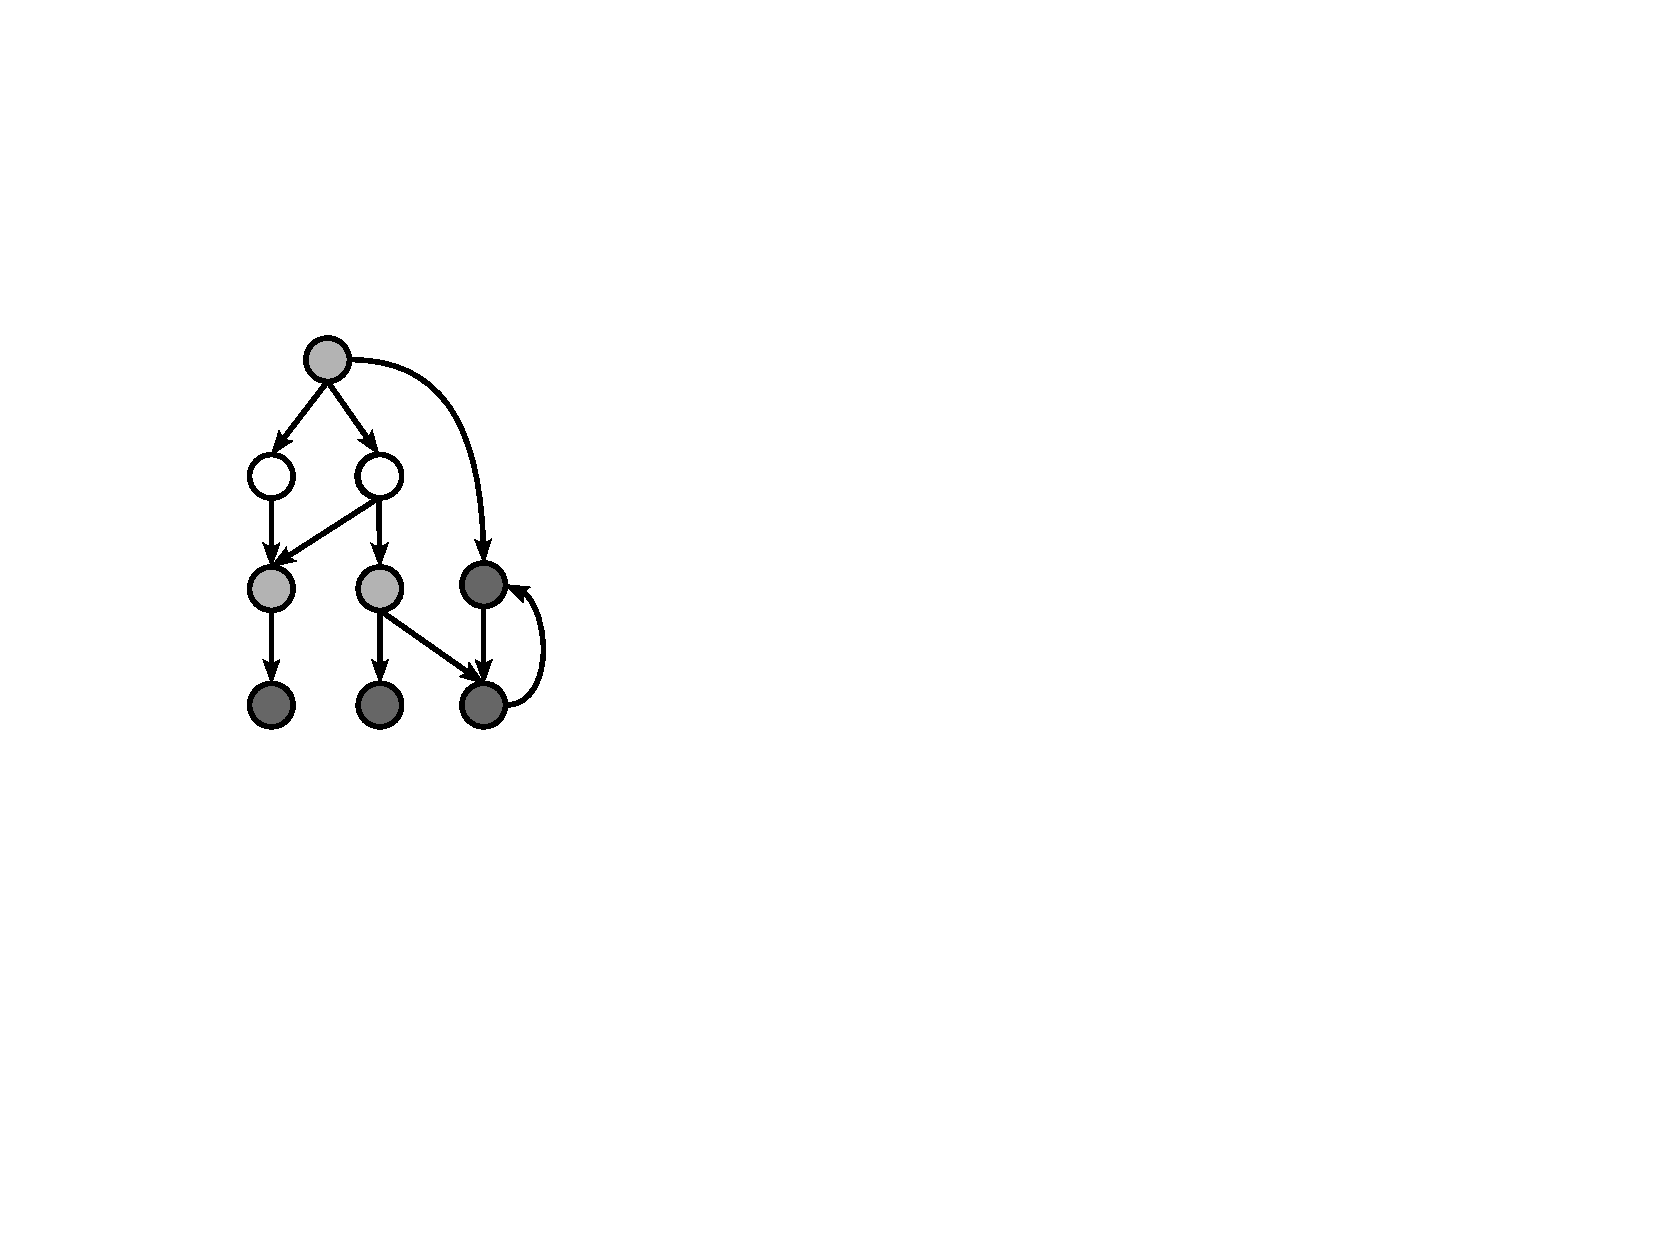
\includegraphics[width=0.3\textwidth]{part4/Figures/exampleGraph}
	\\ \vspace{5mm}
	}
}
\begin{subfloat}
\begin{minipage}[b]{0.65\textwidth}
\begin{shortlisting}
enum Color {
	White, LightGray, DarkGray
}
interface Graph {
	Set<Node> getNodes();
	Set<Edge> getEdges();
}
interface Node {
	Color getColor();
	List<Node> getChildren();
	List<Node> getParents();
}
interface Edge {
	Node getFrom();
	Node getTo();
}
\end{shortlisting}
\end{minipage}
\caption{Abstract data types for nodes and edges.}
\end{subfloat}
	\caption{An example generic graph of three colors of nodes.}
	\label{fig:exampleGraph}
\end{figure}

The first implementation of the \class{Node} and \class{Edge} data types that
comes to mind is a straightforward


\section{Breaking the Java Mold}
\label{sec:fortran-style}

\subsection{The Bulk Sharing Pool}
\label{sec:bulk-sharing-pool}

The bulk storage that backs a set of data items, each of the same type. Objects
share the data by indexing into the pool.

\section{Memory Mapping and Marshalling}